\chapter{La classe P} \label{ch:capitolo10}
\subsection{La classe P}
\textbf{Definizione}\\
Denotiamo con P la classe dei problemi S accettati da una macchina di Turing M tale che $c_M (n) = O(n^k)$ per qualche intero positivo k.\\\\
\textbf{Osservazione}\\
Se $S \in P$, allora c’è una macchina di Turing che, per ogni input w di lunghezza n, si comporta nel modo seguente:
\begin{itemize}
    \item se $w \in S$, allora M accetta w in al più $cl(w)^k$ passi (con c, k costanti positive fissate)
    
    \item se $w \notin S$, allora M $\uparrow$ w
\end{itemize}
In realtà, c’è anche una macchina di Turing M' che decide S con $c_M'(n) = O(n^k)$.
\subsection{2Col}
\textbf{Definizione}\\
Un grafo $G = (V , E)$ è 2-colorabile se esiste una funzione $c : V \mapsto \{1, 2\}$ tale che per ogni $(v, w) \in E$, $f(v) \neq f (w)$.\\
La classe dei grafi 2-colorabili è denotata 2COL.\\\\
\textbf{Proposizione}\\
2COL $\in$ P.\\\\
\textbf{Dimostrazione}\\
È sufficiente trovare un algoritmo che risolve 2COL in tempo polinomiale.\\
\begin{figure}[htp]
    \centering
    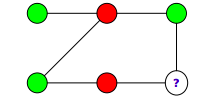
\includegraphics[scale=0.9]{tesi_stile/img/foto1cap10.png}
\end{figure}
\subsection{Algoritmo}
Su input G.
\begin{figure}[htp]
    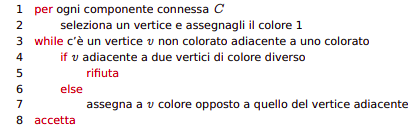
\includegraphics[scale=0.9]{tesi_stile/img/foto2cap10.png}
\end{figure}
\subsection{SAT}
Siano $x_0, x_1, x_2,...$una famiglia, potenzialmente infinita di variabili. Chiameremo letterali le variabili $x_i$ e le loro negazioni $\bar{x}_i$. Una clausola è una sequenza di letterali che non contiene letterali col
medesimo indice.\\
Un sistema di clausole si dice soddisfacibile se esiste una clausola che le interseca tutte (ossia contiene un letterale di ogni clausola del sistema) La famiglia dei sistemi di clausole soddisfacibili è denotata con SAT.\\\\
\textbf{Esempio}\\
Il sistema.
\begin{center}
    $\{(x_0 + \bar{x}_1)(x_0 + \bar{x}_1 + x_2)(x_3 + x_4 + \bar{x}_0)(\bar{x}_4 + \bar{x}_5)\}$
\end{center}
Una clausola che soddisfa il sistema non è altro che un implicante dell’espressione medesima.
Quindi un sistema è soddisfacibile se la corrispondente espressione Booleana non è nulla.
\subsection{2SAT}
\textbf{Definizione}\\
Una clausola di lunghezza 2 si dice 2-clausola.\\
L’insieme dei sistemi di 2-clausole soddisfacibili si denota con 2SAT.\\
\textbf{Proposizione}\\
2SAT $\in$ P.\\\\
\textbf{Dimostrazione}\\
Dobbiamo trovare un algoritmo che risolve 2SAT in tempo polinomiale.\\\\
\textbf{Esempio}\\
\begin{figure}[htp]
    \centering
    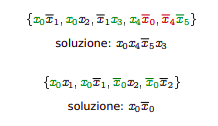
\includegraphics[scale=0.9]{tesi_stile/img/foto3cap10.png}
\end{figure}
\newpage
\subsection{Ridurre 2COL a 2SAT}
Costruiamo una riduzione di 2COL a 2SAT.\\
Devo costruire una funzione calcolabile totale f che a ogni grafo G associa un sistema di 2-clausole f (G) tale che.\\
foto.\\
Sia G = (V , E) un grafo.\\
Per ogni vertice $v_i,i = 1, . . . , n$, introduco una variabile $x_i$ ($x_i$ = "$v_i$ ha colore verde") e per ogni lato $(v_i, v_j) \in E$, le due clausole
\begin{center}
    $x_i, x_j, \bar{x}_i, \bar{x}_j$
\end{center}
(uno dei vertici ha colore verde, uno non ha colore verde).\\\\
\textbf{Algoritmo alternativo per 2COL}\\
Su input G
\begin{figure}[htp]
    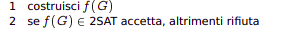
\includegraphics[scale=0.9]{tesi_stile/img/foto4cap10.png}
\end{figure}
\newpage
\subsection{Equazioni lineari}
\textbf{Probelma}\\
\textbf{Input}: Un'equazione $ax + by = c$ con $a, b, c \in Z$
\\\textbf{Output}: si se l’equazione ha una soluzione intera, no altrimenti.\\\\
\textbf{Osservazione}
\begin{itemize}
    \item Se MCD(a, b) = 1, l’equazione ha soluzione intera (teorema di Bezout)
    
    \item Se MCD(a, b) divide c, ci si può ricondurre al caso precedente
    
    \item Se l’equazione ha una soluzione intera, allora MCD(a, b) divide c.
    
\end{itemize}
\textbf{Soluzione}\\
Per risolvere il problema basta calcolare MCD(a, b) e verificare se divide c.\\
Sono necessarie
\begin{itemize}
    \item $O(n^2)$ divisioni, n = $\log_2$ (max$\{a, b, c\}$)
    
    \item Per ogni divisione, $O(n)$ sottrazioni
    
    \item Per ogni sottrazione $O(n)$ operazioni elementari sui bit.
    
    \item totale: $O(n^4)$ operazioni elementari: il problema è nella classe P
\end{itemize}
\newpage
\subsection{Numeri primi}
\textbf{Problema}\\
\textbf{Input:} Un numero a $\in$ N.\\
\textbf{Output:} Si se a è primo, no altrimenti.\\\\
\textbf{Soluzione}\\
Dividi a per tutti gli interi $q = 2, 3,..,|\sqrt{a}|$.
\begin{itemize}
    \item ma sono $|\sqrt{a} - 1| =$ $O(2^{n/2})$ divisioni, $n = \log_2$a
\end{itemize}
L’algoritmo di Agrawal, Kayal, Saxena (2002), ha complessità $O(n^11)$.
Quindi il problema è nella classe P.\\\\
\textbf{Osservazione}\\
Nella pratica, la complessità $n^11$ è troppo alta, per cui per la ricerca di grandi primi si preferiscono algoritmi probabilistici.\\\\
\textbf{Problema}
\textbf{Input:} Un numero $a \in N$.\\
\textbf{Output:} la decomposizione di a in fattori primi.
\subsection{coP}
\textbf{Definizione}\\
Denotiamo coP la classe dei problemi il cui complemento è in P.\\\\
\textbf{Proposizione}\\
coP = P.\\\\
\textbf{Dimostrazione}\\
Se $S \in coP$, c’è una macchina di Turing M che decide S con $c_M(n) = O(n^k)$, per k opportuno.\\
Ma allora c’è una macchina M' che accetta S, con $c_M'(n) = c_M(n) = O(n^k)$\\


(basta aggiungere le istruzioni affinchè M con output SI inizi un loop infinito).



